\section{Proposed method}
\label{sec:method}
\subsection{Problem formulation}
Let $\mathcal D_s=\{(w_i,y_i,d_i)\}_{i=1}^{N_s}$ contain labeled vibration
windows from the observed source conditions, where $y_i\in\{1,\ldots,K\}$
is a fault label and $d_i\in\{1,\ldots,D\}$ identifies a source condition.
The objective is to train a classifier that diagnoses an unseen condition
using only its vibration window. Target signals, labels, rotational speeds,
and target-batch statistics are not inputs to the training algorithm.
Recorded source speeds and sampling rates are used by an offline source
analyzer. The analyzer and its source partners are not needed at deployment.

The fixed two-rate implementation is denoted Q2.
The proposed training construction acts on source observations before
feature extraction. It modifies the timing and effective impulse strength
of an estimated event component while retaining the response kernels and the
unexplained part of the observation. A factual training branch remains in
the classification objective throughout training.

Figure~\ref{fig:framework} summarizes the offline analyzer, source-training
path and deployment path. The editor changes the training distribution;
it adds no inverse solver or source-matching step to deployment.
\begin{figure}[pos=htbp]
\centering
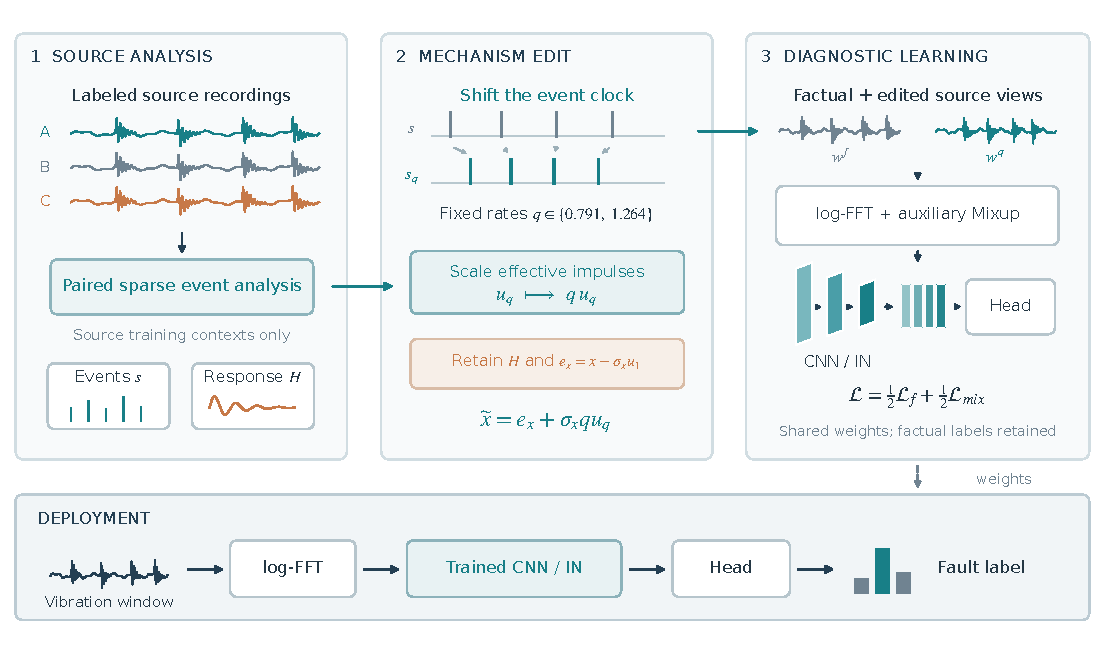
\includegraphics[width=\linewidth]{framework_publication.pdf}
\caption{Observation-anchored event-mechanism editing. Source analysis estimates events and response kernels. The intervention changes event timing and effective strength while retaining the response and observation-anchored remainder. Factual and edited views train one shared network; deployment uses the frontend and classifier only. Traces and feature blocks illustrate the processing stages and are not experimental measurements.}
\label{fig:framework}
\end{figure}


\subsection{Source event analysis}
For a source context $x\in\mathbb R^N$, write
$\bar x=(x-\mu_x)/\sigma_x$, where $\mu_x$ and $\sigma_x>0$ are its saved
source mean and scale. The source analyzer fits a nonnegative event model
together with harmonic and stationary terms:
\begin{equation}
 \bar x_j=H_js_j+A_jb_j+Fc_j+\epsilon_j,\qquad s_j\geq0,
 \quad j\in\{1,2\}.
 \label{eq:analysis}
\end{equation}
Here $j$ indexes two legal source contexts, $H_j$ is a finite convolution
dictionary, $A_j$ contains the first four recorded shaft harmonics, and $F$
contains stationary sinusoidal candidates estimated from the source pair.
Each response dictionary contains four source spectral carrier candidates,
three decay values, and four phases, giving 48 response modes per context.
These modes are analysis kernels; they do not mask frequency bands in the
classifier input.

The sparse inverse minimizes a squared reconstruction term with
nonnegative $\ell_1$ penalties on $s_j$ and group penalties on the sinusoidal
coefficients:
\begin{equation}
 \min_{\substack{s_1,s_2\geq0\\b_1,b_2,c_1,c_2}}
 \frac12\sum_{j=1}^{2}
 \|\bar x_j-H_js_j-A_jb_j-Fc_j\|_2^2
 +\sum_{j=1}^{2}\lambda_{s,j}\|s_j\|_1
 +\lambda_b\|B\|_{2,1}
 +\lambda_c\|C\|_{2,1}.
 \label{eq:inverse}
\end{equation}
A group in $B$ or $C$ contains the corresponding sine and cosine
coefficients across the two source contexts. Fixed proximal iterations
produce the offline coefficients and kernels used to construct the source
bank using accelerated proximal updates \cite{fista}. The classifier does not
backpropagate through this numerical inverse.

Source labels are used when selecting same-class source pairs, even though
Eq.~\eqref{eq:inverse} has no classification loss. The current PU pairing
also preserves the recorded bearing identity. A verified entity identity
is not assumed for PHM or JNU. Both contexts must belong to the current
source-training role; a source-validation or target context cannot serve
as an analysis partner.

\subsection{Observation-anchored mechanism editing}
For one analyzed context, let $s_b[n]$ denote its event coefficients and
$h_b$ its finite response kernels. A kernel is zero outside $[0,L-1]$.
Using the context center $m=(N-1)/2$, define a relative event-rate
transformation
\begin{equation}
 u_q[t]=\sum_{b=1}^{48}\sum_{n=0}^{N-1}
 s_b[n]\,
 h_b\!\left(t-m-\frac{n-m}{q}\right),\qquad q>0.
 \label{eq:render}
\end{equation}
Thus event locations move from $n$ to $m+(n-m)/q$ while the response
shape remains fixed. Fractional lags are evaluated from the same finite
analytic kernel used at $q=1$; they are not created by resampling the
complete recorded waveform. The implementation evaluates $u_1$ and
$u_q$ using the same float64 rendering definition and checks context support
before extracting a query window.

Define the observation-anchored remainder by
\begin{equation}
 e_x=x-\sigma_xu_1 .
 \label{eq:remainder}
\end{equation}
The coupled edit is
\begin{align}
 \mathcal T_q(x)
   &=e_x+\sigma_xq u_q \nonumber\\
   &=x+\sigma_x(q u_q-u_1).
 \label{eq:edit}
\end{align}
The remainder includes the source mean and all components not represented
by $\sigma_xu_1$. It is retained rather than assigned to a disposable
condition branch. Consequently, the method does not require every
condition-dependent feature to be estimated and subtracted.

The relative rate $q$ changes event density and the factor $q$ in
Eq.~\eqref{eq:edit} changes effective event impulse strength. The fixed
coupling rule scales effective impulses linearly with relative rate.
Waveform energy also depends on event overlap, finite support and the
retained remainder.

The implementation returns $\mathcal T_1(x)=x$ exactly. For other values,
the edited query is obtained by cropping the transformed context,
$w^{\,q}=P_r\mathcal T_q(x)$, using the original query location $r$.
No new response or event inverse is fitted for each edit. The current
Q2 recipe samples the two fixed values
\begin{equation}
 q\in\left\{\exp\!\left(-\frac{\log(1.5)}{\sqrt3}\right),
                 \exp\!\left(\frac{\log(1.5)}{\sqrt3}\right)\right\}
       \approx\{0.791286,\;1.263765\}
 \label{eq:q}
\end{equation}
with equal probability. These factors are the same across datasets and are
not chosen from a target rotational speed.

The intervention variables in this event model are event location and
effective impulse strength, with the response and remainder held fixed.
Its utility is tested by matched timing-only, amplitude-only,
global-moment and unedited-bank controls.

The causal motivation is expressed within this event-generation model.
Writing $x=\sigma_x\mathcal H(s)+e_x$, the action changes the estimated
event locations and impulses, while the analyzed response $\mathcal H$ and
observation term $e_x$ are held fixed. Keeping the training label assumes that
the chosen local event changes preserve the diagnostic category. This is a
modeling assumption tested through the learning experiments; it does not follow
from reconstruction accuracy alone. Effective impulses can vary with operating
conditions without changing fault location, but the linear coupling in
Eq.~\eqref{eq:edit} is a fixed augmentation rule rather than a universal
load--speed law. The construction therefore specifies which mechanism is
intervened on without assigning every remaining signal component to a
non-causal branch.

\begin{samepage}
The distinction from waveform time scaling follows directly from the
kernel model. Set the time origin at the context center and write
$\tau_n=n-m$. The event edit and a dilation of the original modeled
component then give
\begin{align}
 v_q(t)&=\sum_{b,n}s_b[n]h_b\!\left(t-\frac{\tau_n}{q}\right),
 \label{eq:centered-edit}\\
 v_1(qt)&=\sum_{b,n}s_b[n]h_b\!\left(q\left[t-\frac{\tau_n}{q}\right]\right).
 \label{eq:waveform-dilation}
\end{align}
\end{samepage}
Both move event centers to $\tau_n/q$. Waveform dilation also scales
the time coordinate inside each response kernel. Q2 preserves the
response shape and scales effective impulse strength separately by $q$
in Eq.~\eqref{eq:edit}. These identities concern the continuous kernel
model; subsequent sampling and finite-query cropping produce the training
inputs. The harmonic and stationary terms retained in $e_x$ keep their
observed coordinates, so $q$ parameterizes an edit of the fitted event clock.

\begin{figure}[pos=htbp]
\centering
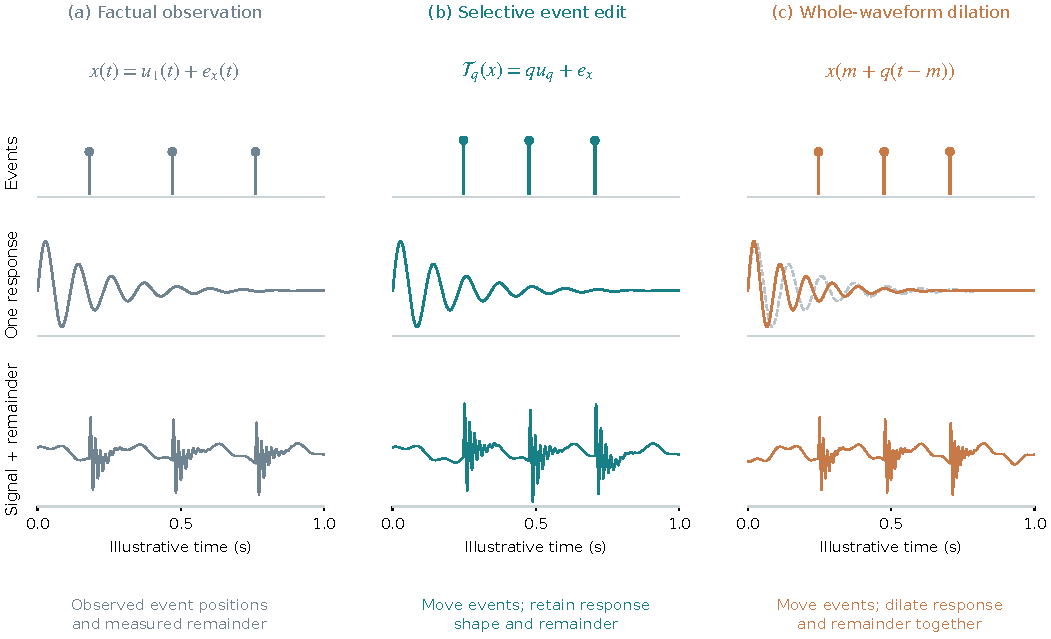
\includegraphics[width=.94\linewidth]{generated/mechanism_publication.pdf}
\caption{Analytic illustration of the operator distinction. Columns show the same three synthetic events under the factual model,
selective editing and whole-waveform dilation. Rows display events, one response
and the resulting observation; dashed traces indicate the original response
or retained background. The illustration uses $q=1.264$ and unit source scale. Q2 moves event centers and scales their impulses while preserving
the response and measured-context term. Whole-waveform dilation also changes
kernel oscillations and background coordinates. This illustration explains
the construction; it is not a measured-signal or classification experiment.}
\label{fig:mechanism}
\end{figure}

\subsection{Classification and feature-space Mixup}
A deterministic frontend $\Phi$ maps each factual or edited query to
$\log(1+|\operatorname{rFFT}(w)|)$, followed by linear interpolation to
2048 frequency positions. A shared convolutional encoder, channel-wise
instance normalization over the feature position axis, and classification
head produce the logits $f_\theta(\Phi(w))$.
Raw-valued queries enter this frontend; the context normalization used by the
offline analyzer is separate from the classifier input transformation.

Training samples are balanced over source-condition and class cells.
For each balanced slot $i$, a factual window $w_i^f$ is drawn from the full
source-training pool and a bank context/query $(x_i^b,r_i)$ is independently
drawn from the same condition and class. They need not come from the same
recording. Their labels agree because of the balanced slot construction;
this is not a requirement to classify one recording using another at test
time.

For a binary edit mask $M_i$, construct the auxiliary feature
\begin{equation}
 a_i =
 \begin{cases}
  \Phi(P_{r_i}\mathcal T_{q_i}(x_i^b)), & M_i=1,\\
  \Phi(w_i^f), & M_i=0 .
 \end{cases}
 \label{eq:aux}
\end{equation}
The mask is sampled with probability $1/2$. At each class and within-cell
position it is shared across source conditions, so that edit activation
does not introduce a different condition-wise sampling rule.
The same sampler and edit-direction streams are used for matched controls.

Mixup acts on the auxiliary features after the log-FFT frontend.
For a batch permutation $\pi$ and a shared
$\lambda\sim\operatorname{Beta}(0.2,0.2)$, let
\begin{equation}
 \widetilde a_i=\lambda a_i+(1-\lambda)a_{\pi(i)} .
 \label{eq:mix}
\end{equation}
The loss combines factual and mixed classification risks:
\begin{align}
 \mathcal L(\theta)
  ={}&\frac{1}{2B}\sum_{i=1}^{B}
       \ell(f_\theta(\Phi(w_i^f)),y_i)\nonumber\\
   &+\frac{1}{2B}\sum_{i=1}^{B}
       \big[\lambda\ell(f_\theta(\widetilde a_i),y_i)
       +(1-\lambda)\ell(f_\theta(\widetilde a_i),y_{\pi(i)})\big],
 \label{eq:loss}
\end{align}
where $\ell$ is cross-entropy.

The network forward concatenates three copies of the factual batch and
three copies of the same mixed batch. Each of the two distinct input
batches therefore occupies $3B$ positions, and the mean risk is
Eq.~\eqref{eq:loss}. Ordinary batch normalization uses this $6B$ layout
during training. All matched operator arms retain the same layout and optimizer schedule.
The locked classifier recipe uses Adam for 2000 updates with learning rate
$10^{-4}$, $(\beta_1,\beta_2)=(0.9,0.999)$ and zero weight decay.

\subsection{Controls and deployment}
The matched operator comparison holds the encoder, normalization, sampler, Mixup,
optimizer and training duration fixed. The strong simple control uses
factual windows for the auxiliary branch. The unedited-bank control
substitutes a clean bank query under the same mask. A timing-only control
uses $x+\sigma_x(u_q-u_1)$ at the endpoints $\{2/3,3/2\}$; another uses
the same two interior values in Eq.~\eqref{eq:q}. The coupled Q2 arm uses
Eq.~\eqref{eq:edit}. The unedited-bank control separates source-bank
sampling from event editing, while the same-rate timing-only control
tests the additional effective-impulse coupling.

Two additional controls test competing amplitude explanations at the same
interior values of $q$. The amplitude-only edit keeps event locations fixed:
\begin{equation}
 \mathcal A_q(x)=x+\sigma_x(q-1)u_1.
 \label{eq:amplitude-control}
\end{equation}
Together with the unedited-bank and same-rate timing-only controls,
this gives four matched arms: unedited, timing-only, amplitude-only and
coupled. For their scores $S_F$, $S_T$, $S_A$ and $S_Q$, the factorial
analysis reports $S_Q-S_A$, $S_Q-S_T$ and the interaction
$S_Q-S_T-S_A+S_F$ using the same metric and weighting.

For a clean query $v=P_rx$ and its coupled edit
$v_Q=P_r\mathcal T_q(x)$, let $\mu(v)$ be the sample mean and
$\rho(v)=\sqrt{N_v^{-1}\sum_t(v[t]-\mu(v))^2}$ its centered RMS.
The global-moment control is
\begin{equation}
 \mathcal M_q(v)=\mu(v_Q)+\frac{\rho(v_Q)}{\rho(v)}[v-\mu(v)].
 \label{eq:moment-control}
\end{equation}
It matches the coupled query's mean and centered RMS before the log-FFT
frontend while preserving the standardized waveform shape. When both
centered RMS values vanish, the control is the constant $\mu(v_Q)$;
a zero clean RMS with a positive edited RMS is rejected rather than
replaced with noise. Zero-event and weak-event queries remain in the
comparison. All controls retain the same source query, label, mask,
Mixup draws and training schedule.

All new source models are frozen before target evaluation.
The 2000-step state is the primary evaluation state; the earliest strict
best among source-validation steps 0, 1000 and 2000 is a secondary analysis.
This reporting policy is not an input to the deployed classifier.
At deployment, a vibration window passes through $\Phi$ and
$f_\theta$ in evaluation mode, with source-trained batch-normalization
running statistics and per-sample instance normalization. The inverse
solver, source partner, $q$, and rotational-speed
metadata are absent from this inference path.
